\section{Lab One: Basic Usage of Infer}

The purpose of this lab is to:
\begin{itemize}
	\itemsep0em
	\item Verify that your Infer installation is working properly by producing \textit{basic reports}.
	\item Generate both HTML and JSON bug reports.
	\item Examine the basic report in a browser and gain familiarity with what basic bug classes 
	Infer finds and how they are reported.
	\item Gain proficiency understanding Infer's reported bugs.
\end{itemize} 

\dothis{Basic Infer Usage}

\vspace{0.5cm}

\textbf{For each of the three targets perform the following operations:}

\begin{enumerate}
	\itemsep0em
	\item In the repo root directory, type:\\
	\verb|make clean|, and then \\
	\verb|infer run --keep-going -- make -j6|\\
    The option \verb|--keep-going| forces the process to keep going when Infer encounters errors. Always recommended. Also, always make sure you have a \verb|make clean| state before analysis.    
    Infer analysis can take some time to complete. Typically:
    \begin{itemize}
    	\item \textbf{Angband}: about 7 minutes
    	\item \textbf{SkyNet}: about 1 minute
    	\item \textbf{BSDGames}: about 3 minutes
    \end{itemize}
	\item When the Infer analysis is complete you will see on screen a summary. 
	Verify that it looks something like the following:\\
	\begin{verbatim}		
		...too many issues to display (limit=10 exceeded), please see
/home/dstcyber/workspace/audit/BSDGames/infer-out/bugs.txt 
or run `infer-explore` for the remaining issues.
		
		Summary of the reports
		
		UNINITIALIZED_VALUE: 100
		DEAD_STORE: 37
		NULL_DEREFERENCE: 34
		RESOURCE_LEAK: 10
		MEMORY_LEAK: 5
		USE_AFTER_FREE: 1		
	\end{verbatim}
	\item Verify that Infer has created a sub-directory containing all its analysis:\\
	\verb|# cd ./infer-out|\\
	Have a look in this directory. If you want to re-run the analysis I tend to just 
	delete the \verb|./infer-out| directory tree and start again. This is not always necessary
	and in fact it can save considerable time if you don't but don't be afraid to delete it if you want 
	to start again.
	\item Inspect the JSON report file:\\
	\verb|# vim ./infer-out/report.json|\\
    You may want to examine this in VSCode which can pretty print format the JSON data. 
	\item Generate a HTML report file:\\
	\verb|# infer explore --html| \\
	You should see something like the following:
	\begin{verbatim}
		Detected GitHub project vattam/BSDGames
		Saved html report in:
		./infer-out/report.html/index.html
	\end{verbatim}
	\item Open the HTML report in a browser \textbf{from your host}:\\
	\verb|# xdg-open ./infer-out/report.html/index.html|
\end{enumerate}

When you open the report in a browser you should see something similar to Figure \ref{fig:screen-one}.
It's not a very attractive looking report  :-)

\begin{figure}
	\centering
	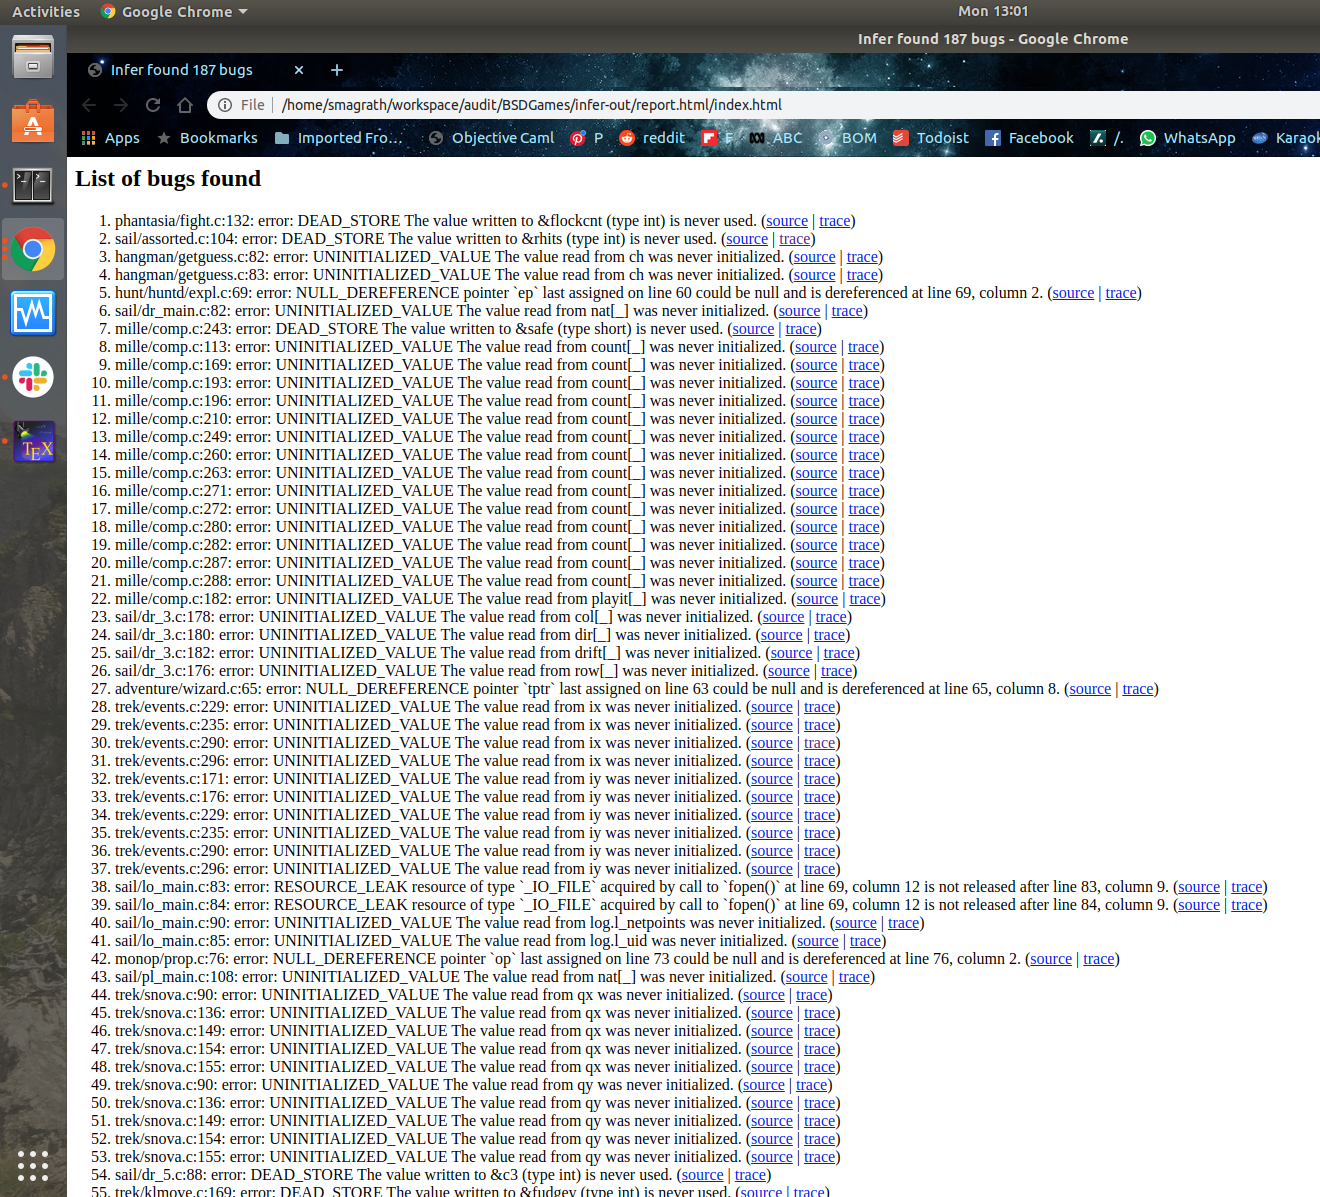
\includegraphics[width=\linewidth]{./img/screen-one}
	\caption[Basic Report]{Basic Infer Report for BSDGames}
	\label{fig:screen-one}
\end{figure}

\vspace{1cm}

\subsection{Examining Bug Reports}

It is very common to get a large number of bug reports when using Infer. 
It is important to have a strategy when deciding which reports to look at.
Your strategy will depend on what your goals are and will improve with experience
in using the tool. Not all bug reports are of equal value.

Your strategy may include factors such as:
\begin{itemize}
	\item Which bug classes are of the most interest to you;
	\item Which functions and translation units (files) are most important;
	\item How much time you have :-)
\end{itemize}

In general, your analysis process will need to examine the \textit{trace} of a bug report.
The trace is a \textit{almost} human readable description of why Infer thinks it has found a bug.
When looking at the trace the most important parts are the \textit{first few lines and the last few lines}. The first line declares what the bug is and where it is. 
The last few lines point to the specific problem point. 
If the trace has reasonable length then the intermediate parts of the trace 
are the execution path which causes the problem. 

\exercise{Click on a sample of the following bug classes:}

\begin{itemize}
	\itemsep0em
	\item \verb|DEAD_STORE|
	\item \verb|NULL_DEREFERENCE|
	\item \verb|UNINITIALIZED_VALUE|
	\item \verb|RESOURCE_LEAK|
	\item \verb|NULL_DEREFERENCE|
	\item \verb|MEMORY_LEAK|
	\item \verb|USE_AFTER_FREE|
\end{itemize}

\textbf{For each of the bug classes consider the following:}
\begin{enumerate}
	\item Is the bug report correct?
	\item If not, can you think of a reason why it failed? \\
	This is an important skill for learning how to quickly dismiss bug reports.
\end{enumerate}


In particular examine the following interesting \textit{specific} bugs:
\begin{itemize}
    \item See the whiteboard :-)
\end{itemize}


However it is important that you learn how to:
\begin{enumerate}
	\item efficiently triage the report when you have a lot of records;
	\item efficiently follow the reasoning of an Infer report trace. 
\end{enumerate}

\subsection{What Have We Learnt So Far?}

\begin{enumerate}
	\itemsep0em
	\item How to install and run Infer using the default checkers;
	\item How to check the Infer man page and online documentation;
	\item The location and contents of the Infer analysis in \verb|./infer-out|
	\item How to find the JSON bug report;
	\item How to generate a HTML report of the bugs found;
	\item How to read the bug traces for a variety of bug classes;
\end{enumerate}

\subsection{What Next?}

In the next lab we will be looking at Integer bugs and Buffer-overflows.


